\documentclass[border=7pt]{standalone}

%\documentclass{article}
\usepackage{tikz}
\begin{document}

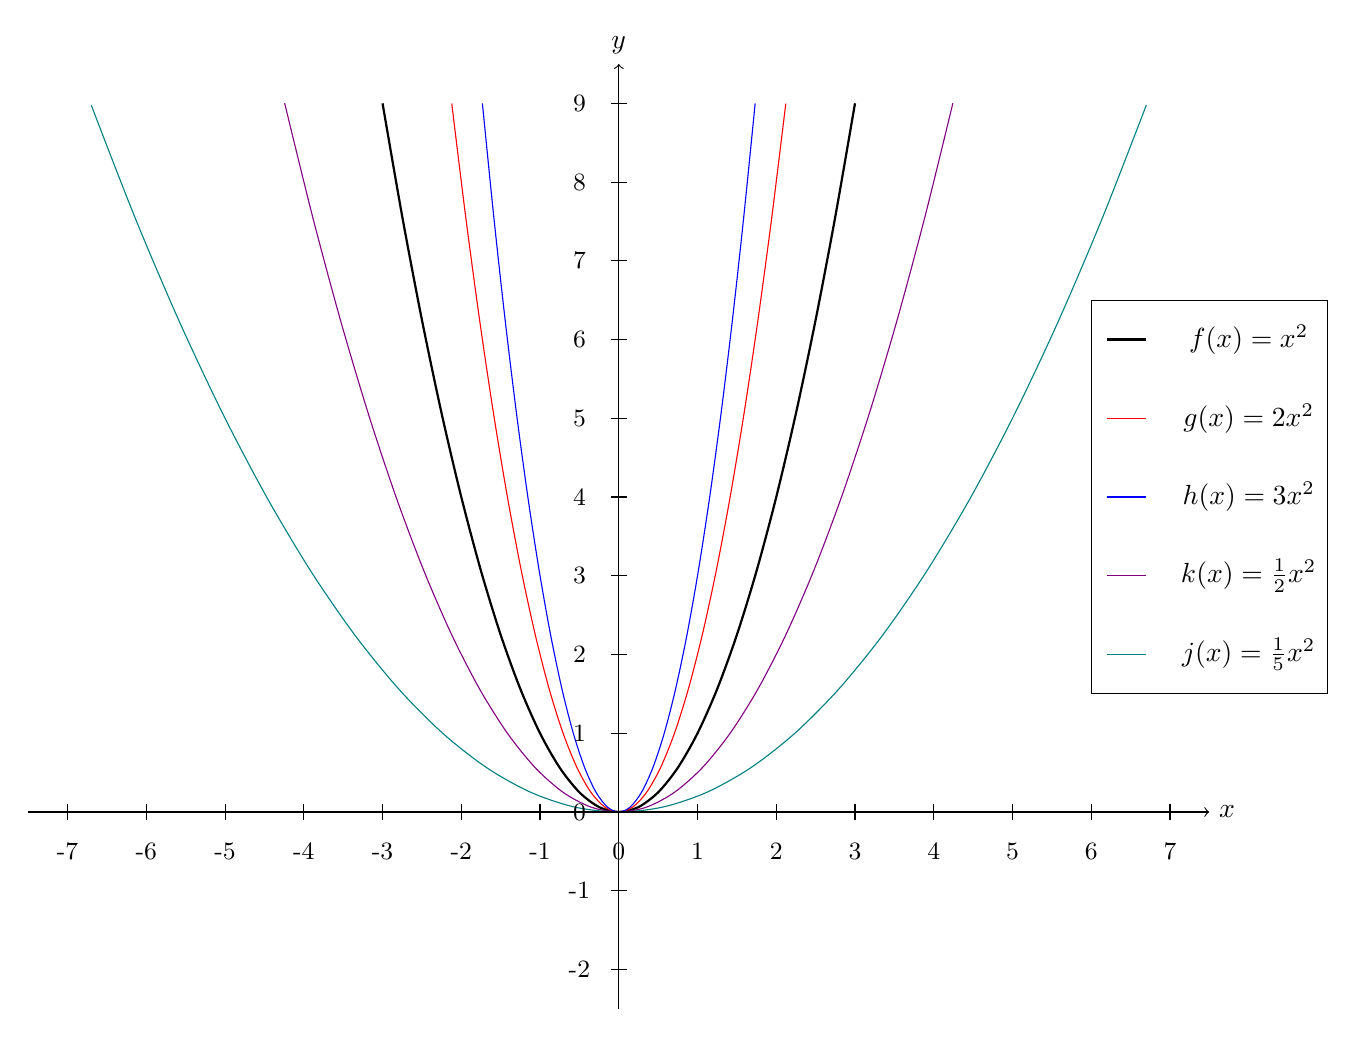
\begin{tikzpicture}

\draw[thick,domain=-3:3,smooth,variable=\x,black] plot ({\x},{\x*\x});
\draw[domain=-2.121:2.121, smooth, variable=\x,red] plot({\x},{2*(\x)^2 });
\draw[domain=-1.732:1.732,smooth,variable=\x,blue] plot ({\x},{3*(\x)^2 });
\draw[domain=-4.243:4.243, smooth, variable=\x,violet] plot({\x},{.5*(\x)^2 });
\draw[domain=-6.7:6.7, smooth, variable=\x,teal] plot({\x},{.2*(\x)^2 });

\node (c) at (8,6) {$f(x)=x^2$};
\node (c) at (8,5) {$g(x)=2x^2$};
\node (c) at (8,4) {$h(x)=3x^2$};
\node (c) at (8,3) {$k(x)=\frac{1}{2} x^2$};
\node (c) at (8,2) {$j(x)=\frac{1}{5} x^2$};
\draw[black, thick] (6.2,6) -- (6.7,6);
\draw[red] (6.2,5) -- (6.7,5);
\draw[blue] (6.2,4) -- (6.7,4);
\draw[violet] (6.2,3) -- (6.7,3);
\draw[teal] (6.2,2) -- (6.7,2);
\draw (6,6.5)--(9,6.5)--(9,1.5)--(6,1.5)--(6,6.5);

\draw[->] (-7.5,0) -- (7.5,0) node[right] {$x$};
\draw[->] (0,-2.5) -- (0,9.5) node[above] {$y$};

\foreach \x in {-7,-6,-5,-4,-3,-2,-1,0,1,2,3,4,5,6,7}{
     \draw (\x,-0.5) node{\small\x};
     \draw (\x,-0.1) -- (\x,0.1);
     };

\foreach \x in {-2,-1,0,1,2,3,4,5,6,7,8, 9}{
  \draw (-0.5,\x) node{\small\x};
  \draw (-0.1,\x) -- (0.1,\x);
  };

\end{tikzpicture}
\end{document}
